\def\COMMITINFOS{}
\documentclass[fr]{../../../../../../eplexam}
\usepackage{mathtools}
\DeclareMathOperator{\rang}{\mathrm{rang}}
\usepackage{systeme}

\hypertitle{Signaux et systèmes}{4}{FSAB}{1106}{2016}{Juin}{All}
{Louis Devillez\and Gilles Peiffer}
{Luc Vandendorpe et Vincent Wertz}
\section{Question 1: LV}
On s'intéresse à une forme plus générale du théorème d'échantillonnage. Dans la forme ``classique'', les échantillons d'un signal $x_{\textnormal{a}}(t)$ de départ, en temps continu, sont pris en des instants $nT$ où $T$ est la période d'échantillonnage. Cela donne naissance au signal $x_{\textnormal{e}}(t)$ donné par
\[ x_{\textnormal{e}}(t) = \sum_{n=-\infty}^{+\infty} x_{\textnormal{a}}(nT)\delta(t-nT).\]
On s'intéresse au résultat de l'échantillonnage lorsque les échantillons sont pris en des positions $nT + T_0$ avec $T_0$ quelconque.
\begin{enumerate}
	\item Donnez l'expression du signal échantillonné $x_{\textnormal{e,}T_0}$ résultant.
	\item Donnez l'expression de $X_{e,T_0}(\imagj \omega)$, le spectre de $x_{\textnormal{e,}T_0}$, en fonction de $X_{\textnormal{a}}(\imagj \omega)$, le spectre de $x_{\textnormal{a}}(t)$.
	\item Lorsque vous additionnez $x_{\textnormal{e}}(t)$ et $x_{\textnormal{e,}T_0}$ avec $T_0 = T/2$, qu'obtenez-vous comme signal? Donnez-en l'expression analytique et faites un graphe de ce signal. Vérifiez votre résultat en regardant ce qu'il en est de $X_{\textnormal{e,}0}(\imagj \omega) +X_{\textnormal{e,}T_0/2}$.
\end{enumerate}

\begin{solution}
	\begin{enumerate}
		\item \[x_{\textnormal{e,}T_0}= \sum_{n=-\infty}^{+\infty} x_{\textnormal{a}}(nT + T_0)\delta(t-nT-T_0).\]
		\item
		Pour cela, on multiplie notre signal $x_{\textnormal{a}}(t)$ par un peigne de Dirac positionné en $T_0 + nT$ :
		\begin{align*}
		p(t) &= \sum_{n=-\infty}^{+\infty} \delta(t-nT-T_0) \\
		\textnormal{FS : }\quad P[k] &= \frac{1}{T} \int_{T} y(t) \e^{-\frac{2\pi \imagj k t}{T}}. \\
		\shortintertext{Sur une période $T$, par exemple celle qui contient $T_0$ :}
		&= \frac{1}{T} \int_{T} \delta(t-T_0) \e^{-\frac{2k\pi \imagj t}{T}} = \frac{1}{T} \e^{-\frac{2k\pi \imagj T_0}{T}} \\
		\implies P(\imagj \omega) &= \frac{2\pi}{T} \sum_{k=-\infty}^{+\infty} \e^{-2k\pi \imagj\frac{T_0}{T}} \delta\left(\omega-\frac{2k\pi}{T}\right).
		\end{align*}
		En multipliant $x_{\textnormal{a}}(t)$ par le peigne en temporel, on obtient en fréquentiel :
		\begin{align*}
		x_{\textnormal{e,}T_0}(t) = x_{\textnormal{a}}(t)p(t) \longleftrightarrow X_{e, T_0}(\imagj \omega) &= \frac{1}{2\pi} X_{\textnormal{a}}(\imagj \omega) \ast \left( \frac{2\pi}{T} \sum_{k=-\infty}^{+\infty} \e^{-2k\pi \imagj\frac{T_0}{T}} \delta\left(\omega-\frac{2k\pi}{T}\right) \right) \\
		&= \frac{1}{T} \sum_{k=-\infty}^{+\infty} X_{\textnormal{a}}(\imagj \omega) \ast \delta\left(\omega-\frac{2k\pi}{T}\right) \e^{-2k\pi \imagj\frac{T_0}{T}} \\
		&= \frac{1}{T} \sum_{k=-\infty}^{+\infty} X_{\textnormal{a}}\left(\imagj\left(\omega-\frac{2k\pi}{T}\right)\right) \e^{-2k\pi \imagj\frac{T_0}{T}}.
		\end{align*}
		La dernière égalité venant du fait que $\delta$ est le neutre de la convolution\footnote{Sinon,
		\begin{align*}
		X_{\textnormal{a}}(\imagj \omega) \ast \delta\left(\omega-\frac{2k\pi}{T}\right) &= \int_{-\infty}^{+\infty} X_{\textnormal{a}}(\imagj\gamma) \delta\left(\gamma-\left(\omega-\frac{2k\pi}{T}\right)\right) \dif{\gamma} \\
		&= X_{\textnormal{a}}\left( \imagj \left(\omega-\frac{2k\pi}{T}\right) \right).
		\end{align*}
		}.

		\item
		\begin{align*}
		x_{\textnormal{e,}0} + x_{\textnormal{e,}T/2} &= \sum_{n=-\infty}^{+\infty} x_{\textnormal{a}}(nT)\delta(t-nT) + x_{\textnormal{a}}(nT + T/2)\delta(t-nT-T/2) \\
		&=\sum_{n=-\infty}^{+\infty} x_{\textnormal{a}}(nT/2)\delta(t-nT/2),
		\end{align*}
		soit le signal $x_{\textnormal{a}}(t)$ échantillonné à une fréquence double. Voyons ce qu'il en est de la transformée (en notant $\omega_0=\frac{2\pi}{T}$) :
		\begin{align*}
		\mathcal{F}\{x_{\textnormal{e,}0}(t) + x_{\textnormal{e,}T/2}(t)\} &= X_{\textnormal{e,}0}(\imagj \omega) + X_{\textnormal{e,}T/2}(\imagj \omega) \\
		&= \frac{1}{T} \sum_{k=-\infty}^{+\infty} X_{\textnormal{a}} \left(\imagj\left( \omega-k\omega_0 \right)\right) + \frac{1}{T} \sum_{k=-\infty}^{+\infty} X_{\textnormal{a}} \left(\imagj\left( \omega-k\omega_0 \right)\right) \e^{-2k\pi \imagj\frac{T/2}{T}} \\
		&= \frac{1}{T} \sum_{k=-\infty}^{+\infty} X_{\textnormal{a}} \left(\imagj\left( \omega-k\omega_0 \right)\right) (1-\e^{-k\pi \imagj})\\
		 &= \frac{1}{T} \sum_{k=-\infty}^{+\infty} X_{\textnormal{a}} \left(\imagj\left( \omega-k\omega_0 \right)\right)(1-(-1)^k) \\
		&= \frac{1}{T} \sum_{k=-\infty\textnormal{, } k\text{ pair}}^{+\infty} 2 X_{\textnormal{a}} \left(\imagj\left( \omega-\frac{2k\pi}{T} \right)\right) \\
		&= \frac{1}{T/2} \sum_{k'=-\infty}^{+\infty} X_{\textnormal{a}} \left(\imagj\left( \omega-\frac{2k'\pi}{T/2} \right)\right).
		\end{align*}
		soit le spectre de l'échantillonnage de $x_{\textnormal{a}}(t)$ à une fréquence double, ce qui est assez vraisemblable.
		\begin{center}
			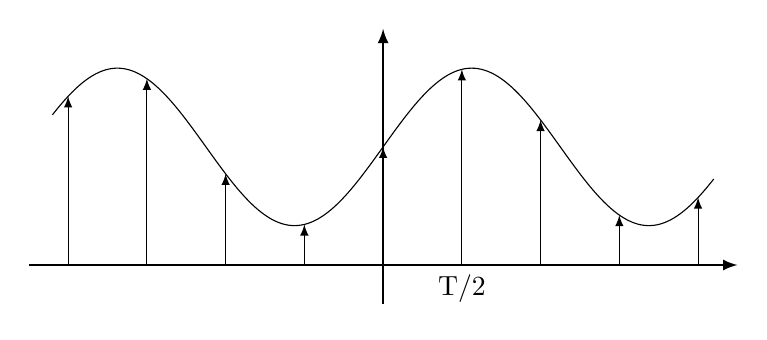
\begin{tikzpicture}
			\draw [thick,-latex](-4.5,0) -- (4.5,0);
			\draw [thick,-latex] (0,-0.5) -- (0,3);
			\draw [domain=-4.2:4.2,samples =200] plot(\x,{1.5+sin(80*\x)});
			\foreach \r in {-4,...,4}
			{
				\draw [-latex] (\r,0)	-- (\r,{1.5+sin(\r*80)});
			}
			\draw (1,0) node[below]{T/2};
			\end{tikzpicture}
		\end{center}
	\end{enumerate}
\end{solution}
\section{Question 2: LV2}
On s'intéresse à un système où la relation entrée ($x(t)$) - sortie ($y(t)$) est donnée par l'équation différentielle suivante:
\[\frac{\dif^{3}y(t)}{\dif t^{3}} +20 \ffdif{y(t)}{t}+100\fdif{y(t)}{t} = 100 \fdif{x(t)}{t} +100x(t).\]

\begin{enumerate}
	\item Calculez $H(\imagj \omega$), la réponse en fréquence du système.
	\item Calculez la réponse impulsionnelle de ce système. Donnez les valeurs numériques finales apparaissant dans la réponse impulsionnelle.
	\item Dessinez le diagramme de Bode de ce système (module uniquement).
	\item Effectuez dans $H(\imagj \omega$) un changement de variable qui correspond à la transformation d'un filtre passe-bas en filtre passe-haut. Pour le résultat obtenu noté $H_{\textnormal{b}}(\imagj \omega)$, représentez à nouveau le diagramme de Bode.
	\item Si l'on introduit dans le système représenté par $H(\imagj \omega$) un signal donné par $x(t) = \cos(\omega_0t+\phi_0) +0.1\sin(\omega_1t + \phi_1)$, qu'obtient-on comme signal de sortie, $y(t)$?
\end{enumerate}
\begin{solution}
	\begin{enumerate}
		\item
		\[Y(\imagj \omega) ((\imagj \omega)^3 + 20(\imagj \omega)^2 + 100(\imagj \omega)) = X(\imagj \omega) ( 100(\imagj \omega)+100) \]
		\[\implies H(\imagj \omega) = \cfrac{100(\imagj \omega +1)}{\imagj \omega((\imagj \omega)^2+20(\imagj \omega)+100)} = \cfrac{100(\imagj \omega +1)}{\imagj \omega(\imagj \omega+10)^2}.\]

		\item

		 \[H(\imagj \omega) = \cfrac{100(\imagj \omega +1)}{\imagj \omega(\imagj \omega+10)^2} = \cfrac{A}{\imagj \omega} + \cfrac{B}{\imagj \omega+10} + \cfrac{C}{(\imagj \omega+10)^2}\]
		 \begin{align*}
			 \implies
		 \begin{cases}
			 100 &= 100 A \\
			 100 &= 20A + 10B + C \\
			 0 &= A+B
		 \end{cases}
	 	\end{align*}
		\[\implies H(\imagj \omega) = \cfrac{1}{\imagj \omega} + \cfrac{-1}{\imagj \omega+10} + \cfrac{90}{(\imagj \omega+10)^2}\]
		\[\implies y(t) = (1 - \e^{-10t} +90t\e^{-10t}) u(t)\footnote{Si on utilise la transformée de Fourier inverse il faut rajouter le terme $0.5$.}.\]

		\item Diagramme de Bode:

		\begin{center}
			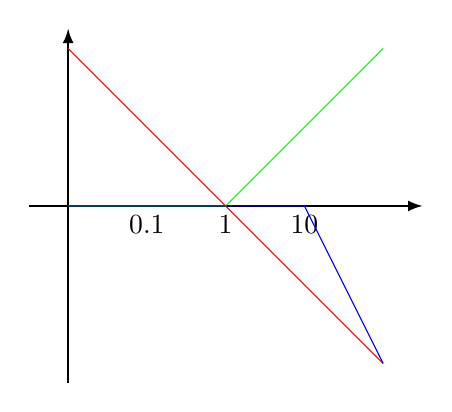
\begin{tikzpicture}
			\draw [thick,-latex] (0,-2.25) -- (0,2.25);
			\draw [thick,-latex] (-0.5,0) -- (4.5,0);
			\draw (1,0) node[below]{0.1};
			\draw (2,0) node[below]{1};
			\draw (3,0) node[below]{10};
			\draw [red] (0,2) -- (4,-2);
			\draw [green](0,0) -- (2,0) -- (4,2);
			\draw [blue] (0,0) -- (3,0) -- (4,-2);
			\end{tikzpicture}
			\begin{tikzpicture}
			\draw [thick,-latex] (0,-2.25) -- (0,2.25);
			\draw [thick,-latex] (-0.5,0) -- (4.5,0);
			\draw (1,0) node[below]{0.1};
			\draw (2,0) node[below]{1};
			\draw (3,0) node[below]{10};
			\draw [red] (0,2) -- (2,0) -- (3,0) -- (4,-2);
			\end{tikzpicture}
		\end{center}

		\item

		\[H_{\textnormal{b}}(\imagj \omega) = H(\frac{1}{\imagj \omega}) \]
		\[H_{\textnormal{b}}(\imagj \omega) = \cfrac{100(\imagj \omega)^2(1+\imagj \omega)}{(1+\imagj \omega10)^2}.\]

		\begin{center}
			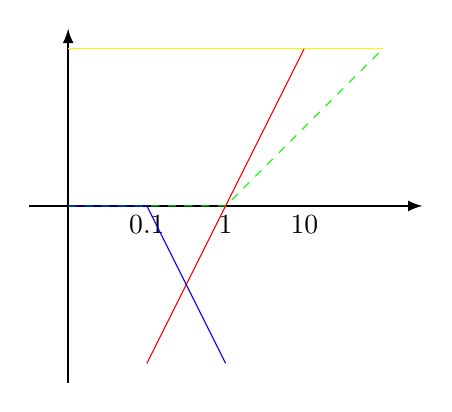
\begin{tikzpicture}
			\draw [thick,-latex] (0,-2.25) -- (0,2.25);
			\draw [thick,-latex] (-0.5,0) -- (4.5,0);
			\draw (1,0) node[below]{0.1};
			\draw (2,0) node[below]{1};
			\draw (3,0) node[below]{10};
			\draw [red] (1,-2) -- (3,2);
			\draw [green,dashed](0,0) -- (2,0) -- (4,2);
			\draw [blue] (0,0) -- (1,0) -- (2,-2);
			\draw [yellow] (0,2) -- (4,2);
			\end{tikzpicture}
			\begin{tikzpicture}
			\draw [thick,-latex] (0,-2.25) -- (0,2.25);
			\draw [thick,-latex] (-0.5,0) -- (4.5,0);
			\draw (1,0) node[below]{0.1};
			\draw (2,0) node[below]{1};
			\draw (3,0) node[below]{10};
			\draw [red] (0,-2) -- (1,-0) -- (2,0) -- (4,2);
			\end{tikzpicture}
		\end{center}
		\item

		\[y(t) =\abs{H(\imagj\omega_0)} \cos(\omega_0t+\phi_0 + \arg{(H(\imagj\omega_0))}) +\abs{H(\imagj\omega_1)}0.1\sin(\omega_1t + \phi_1 + \arg{(H(\imagj\omega_1))}).\]
	\end{enumerate}


\end{solution}

\section{Question 3: VW1}
Soit la transformée de Laplace bilatérale d'une fonction $h(t)$ donnée par:
\[H(s) = \frac{2}{s-1} + \frac{4}{s+2} +\frac{1}{s+3}.\]
\begin{enumerate}
	\item Indiquez toutes les régions de convergence possibles pour cette fonction + justifications.
	\item Dans chaque cas calculez la transformée inverse $h(t)$.
	\item Préciser dans quel(s) cas le système représenté par la réponse impulsionnelle $h(t)$ est BIBO stable.
\end{enumerate}

\begin{solution}
\begin{enumerate}
	\item 	$\mathrm{ROC}$:
	\begin{center}
		\begin{tikzpicture}
			\draw [thick,-latex] (0,-1) -- (0,3);
			\draw [thick,-latex] (-4,0) -- (2,0);
			\draw [dashed] (-3,0) -- (-3,3);
			\draw [dashed] (-2,0) -- (-2,3);
			\draw [dashed] (1,0) -- (1,3);
			\draw [dashed] (-3,-0.5) -- (-3,-1);
			\draw [dashed] (-2,-0.5) -- (-2,-1);
			\draw [dashed] (1,-0.5) -- (1,-1);
			\draw (-3.5,2)node[]{1};
			\draw (-2.5,2)node[]{2};
			\draw (-0.5,2)node[]{3};
			\draw (1.5,2)node[]{4};
			\draw (-3,0)node[below]{-3};
			\draw (-2,0)node[below]{-2};
			\draw (1,0)node[below]{1};
		\end{tikzpicture}
	\end{center}
	\subitem 1
	\[\mathrm{ROC}_1 = \Re\{s\} <1\]
	\[\mathrm{ROC}_2 = \Re\{s\} <-2\]
	\[\mathrm{ROC}_3 = \Re\{s\} <-3\]
	\[\mathrm{ROC} = \Re\{s\} <-3.\]

	\subitem 2
	\[\mathrm{ROC}_1 = \Re\{s\} <1\]
	\[\mathrm{ROC}_2 = \Re\{s\} <-2\]
	\[\mathrm{ROC}_3 = \Re\{s\} >-3\]
	\[\mathrm{ROC} = -3 < \Re\{s\} < -2.\]

	\subitem 3
	\[\mathrm{ROC}_1 = \Re\{s\} <1\]
	\[\mathrm{ROC}_2 = \Re\{s\} >-2\]
	\[\mathrm{ROC}_3 = \Re\{s\} >-3\]
	\[\mathrm{ROC} = -2< \Re\{s\} <1.\]

	\subitem 4
	\[\mathrm{ROC}_1 = \Re\{s\} >1\]
	\[\mathrm{ROC}_2 = \Re\{s\} >-2\]
	\[\mathrm{ROC}_3 = \Re\{s\} >-3\]
	\[\mathrm{ROC} = 1< \Re\{s\}.\]

	\item
	\subitem 1
	\[h(t) = -2\e^{t} u(-t) - 4\e^{-2t} u(-t)-\e^{-3t} u(-t).\]


	\subitem 2
	\[h(t) = -2\e^{t} u(-t) - 4\e^{-2t} u(-t)+\e^{-3t} u(t).\]

	\subitem 3
	\[h(t) = -2\e^{t} u(-t) + 4\e^{-2t} u(t)+\e^{-3t} u(t).\]

	\subitem 4
	\[h(t) = 2\e^{t} u(t) + 4\e^{-2t} u(t)+\e^{-3t} u(t).\]

	\item Seul 3 est BIBO stable puisque sa $\mathrm{ROC}$ contient l'axe imaginaire.

\end{enumerate}
\end{solution}

\section{Question 4: VW2}
Le schéma-bloc suivant illustre un dispositif possible d'atténuation du bruit lorsqu'un pilote d'hélicoptère doit transmettre des informations par radio à une émission d'information sur le trafic routier. La fonction de transfert $H_1$ modélise le canal allant du bruit du moteur ($x$) vers le micro dans lequel s'exprime le pilote. Le signal $w$ est celui émis par la voix du pilote. La fonction de transfert $H_2$ modélise le canal allant du bruit du moteur ($x$) vers un autre micro placé à l'arrière du casque du pilote, et insensible à $w$. La fonction de transfert $H_3$ est conçue comme un filtre atténuant l'effet de $x$ sur le signal envoyé par radio, $y$.
\begin{center}
	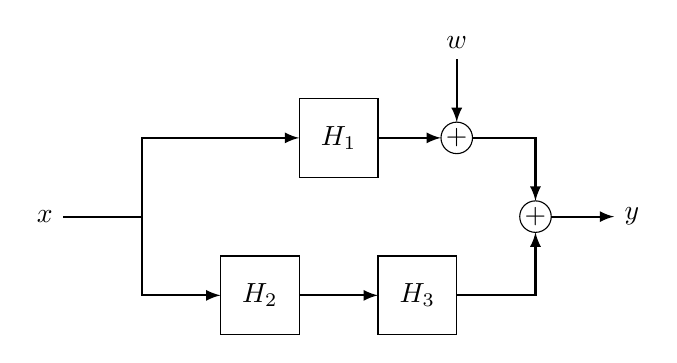
\begin{tikzpicture}
	\draw [thick,-latex] (0,0) node[left]{$x$} -- (1,0) -- (1,1) -- (3,1);
	\draw [thick,-latex] (5,2) node[above]{$w$} -- (5,1.2);
	\draw [thick,-latex]  (1,0) -- (1,-1) -- (2,-1);
	\draw [thick,-latex]  (3,-1) -- (4,-1);
	\draw [thick,-latex]  (5,-1) -- (6,-1) -- (6, -0.2);
	\draw [thick,-latex]  (6.2,0) -- (7,0)node[right]{$y$};
	\draw [thick,-latex] (5.2,1) -- (6,1) -- (6,0.2);
	\draw [thick,-latex] (4,1) -- (4.8,1);
	\draw (3,0.5) rectangle (4,1.5);
	\draw (3.5,1) node[]{$H_1$};
	\draw (2,-0.5) rectangle (3,-1.5);
	\draw (2.5,-1) node[]{$H_2$};
	\draw (4,-0.5) rectangle (5,-1.5);
	\draw (4.5,-1) node[]{$H_3$};
	\draw (6,0) circle(0.2) node[]{+};
	\draw (5,1) circle(0.2) node[]{+};

	\end{tikzpicture}
\end{center}
\begin{enumerate}
	\item Déterminez la fonction de transfert de ce filtre $H_3$.
	\item Expliquez le problème qui se pose si $H_2$ est mal connue et est approximée par une fonction de transfert $H_2$ qui possède un zéro dans le demi-plan de droite.
\end{enumerate}

\begin{solution}
	\begin{enumerate}
		\item Fonction de transfert:
		On voit que
		\begin{align*}
			y &= w + H_1 x + H_2 H_3 x\\
			&= w + (H_1 + H_2 H_3) x.
		\end{align*}
		On veut éliminer le bruit du moteur, c'est-à-dire faire disparaître l'influence
		de $x$.
		Il faut donc que
		\begin{align*}
			 H_1 + H_2 H_3 = 0
		\end{align*}
		ou bien
		 \[H_3 = -\frac{H_1}{H_2}.\]
		\item Il risque de se produire une amplification illimitée du bruit dans la sortie $y$
		car la nouvelle fonction de transfert a un pôle dans le demi-plan de droite, perdant ainsi sa stabilité BIBO.
	\end{enumerate}
\end{solution}

\section{Question 5:VW3}
On considère le filtre représenté par le schéma bloc suivant:

\begin{center}
	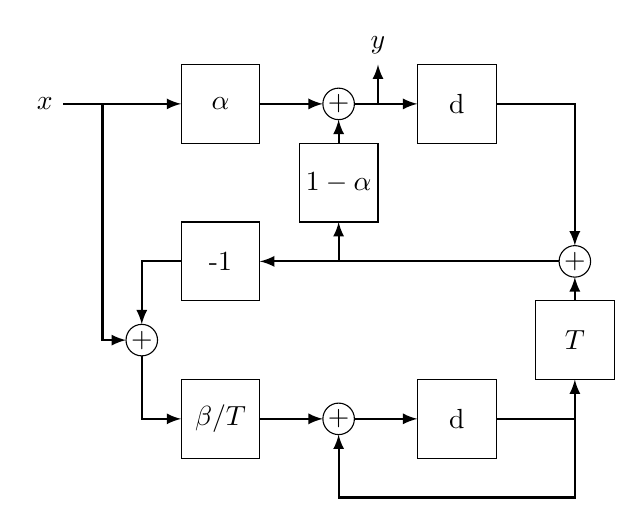
\begin{tikzpicture}
		\draw [thick,-latex] (-0.5,0) node[left]{$x$} -- (1,0);
		\draw [thick,-latex] (2,0)--(2.8,0);
		\draw (1,0.5) rectangle (2,-0.5);
		\draw (1.5,0) node[]{$\alpha$};
		\draw (3,0) circle(0.2) node[]{+};
		\draw  [thick,-latex] (3.2,0) -- (3.5,0) -- (3.5,0.5)node[above]{$y$};
		\draw  [thick,-latex] (3.5,0) --(4,0);
		\draw (4,0.5) rectangle (5,-0.5);
		\draw (4.5,0) node[]{d};
		\draw  [thick,-latex](5,0) -- (6,0) -- (6,-1.8);
		\draw (6,-2) circle(0.2) node[]{+};
		\draw  [thick,-latex] (5.8,-2)  -- (3,-2) -- (3,-1.5);
		\draw (2.5,-1.5) rectangle (3.5,-0.5);
		\draw  [thick,-latex] (3,-0.5) -- (3,-0.2);
		\draw (3,-1) node[]{$1-\alpha$};
		\draw  [thick,-latex] (3,-2) -- (2,-2);
		\draw (1,-1.5) rectangle (2,-2.5);
		\draw (1.5,-2) node[]{-1};
		\draw  [thick,-latex] (1,-2) -- (0.5,-2) --(0.5,-2.8);
		\draw  [thick,-latex] (0,0) -- (0,-3) --(0.3,-3);
		\draw (0.5,-3) circle(0.2) node[]{+};
		\draw  [thick,-latex](0.5,-3.2) -- (0.5,-4) -- (1,-4);
		\draw (1,-3.5) rectangle (2,-4.5);
		\draw (1.5,-4) node[]{$\beta / T$};
		\draw   [thick,-latex](2,-4) --(2.8,-4);
		\draw (3,-4) circle(0.2)node[]{+};
		\draw [thick,-latex] (3.2,-4) -- (4,-4);
		\draw (4,-3.5) rectangle (5,-4.5);
		\draw (4.5,-4) node[]{d};
		\draw  [thick,-latex] (5,-4) -- (6,-4) -- (6,-3.5);
		\draw (5.5,-3.5) rectangle (6.5,-2.5);
		\draw(6,-3) node[]{$T$};
		\draw [thick,-latex] (6,-2.5) -- (6,-2.2);
		\draw  [thick,-latex](6,-4) -- (6,-5) -- (3,-5) -- (3,-4.2);
	\end{tikzpicture}
\end{center}
où d représente l'opérateur de décalage et $\alpha$, $\beta$ et $T$ sont des paramètres réels.
\begin{enumerate}
	\item Donnez une représentation d'état de ce système.
	\item Calculez la fonction de transfert de $x$ vers $y$.
	\item Discutez de l'observabilité et de la commandabilité.
\end{enumerate}
\begin{solution}
\begin{enumerate}
	\item Représentation d'état, avec $q_1[n]$ l'état à la sortie du bloc de décalage du haut, et $q_2[n]$ l'état à la sortie du bloc de décalage du bas :
	\begin{align*}
	\begin{pmatrix}
	q_1\left[n+1\right]\\
	q_2\left[n+1\right]
	\end{pmatrix} &=
	\begin{pmatrix}
		1-\alpha & T(1-\alpha) \\
		-\beta/T & 1 - \beta
	\end{pmatrix}
	\begin{pmatrix}
	q_1\left[n\right]\\
	q_2\left[n\right]
	\end{pmatrix}
	+
	\begin{pmatrix}
	\alpha\\
	\beta / T
	\end{pmatrix}
	x\left[n\right] \\
	y\left[n\right] &=
	\begin{pmatrix}
	1-\alpha & T(1-\alpha)
	\end{pmatrix}
	\begin{pmatrix}
	q_1\left[n\right]\\
	q_2\left[n\right]
	\end{pmatrix}
	+
	\begin{pmatrix}
	\alpha
	\end{pmatrix}
	x\left[n\right].
	\end{align*}

	\item Fonction de transfert:
	\begin{align*}
	H(z) &= C(zI-A)^{-1} B + D\\
	&= \cfrac{z(z\alpha -\alpha + \beta)}{z^2 + z(\alpha + \beta -2) +1 - \alpha}.
	\end{align*}

	\item Commandabilité et observabilité:
	\begin{align*}
	\rang(\mathcal{C}(A,B)) &=
	\rang \begin{pmatrix}
	B & AB
	\end{pmatrix}\\
	&= \rang \begin{pmatrix}
	\alpha & (\alpha + \beta) (1-\alpha)\\
	\beta/T & \frac{\beta}{T}(1-\beta-\alpha)
	\end{pmatrix}\\
	&=\rang \begin{pmatrix}
	\alpha & (\alpha+\beta)(1-\alpha) \\ 0 & \frac{-\beta}{\alpha T} \\
	\end{pmatrix}\\
	\rang(\mathcal{O}(A,C)) &=
	\rang\begin{pmatrix}
	C \\
	CA
	\end{pmatrix}\\
	&=\rang \begin{pmatrix}
	1-\alpha & T(1-\alpha)\\
	(1-\alpha)(1-\alpha - \beta)& T(1-\alpha)(2-\alpha - \beta)
	\end{pmatrix}\\
	&=\rang \begin{pmatrix}
	A-\alpha & T(1-\alpha) \\ 0 & T(1-\alpha) \\
	\end{pmatrix}.
	\end{align*}
	Pour $\beta = 0$ et $T\neq 0$ nous avons une perte de commandabilité car la matrice $\mathcal{C}(A,B)$ n'est pas de plein rang. Si $T=0$, le système se simplifie en
	\begin{center}
		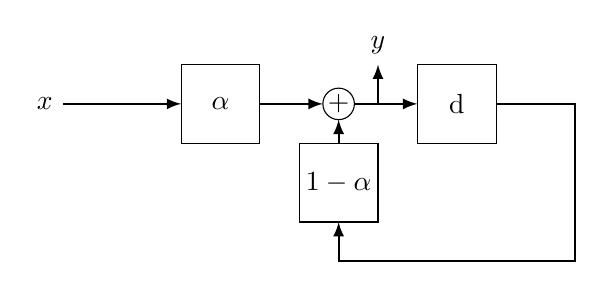
\begin{tikzpicture}
		\draw [thick,-latex] (-0.5,0) node[left]{$x$} -- (1,0);
		\draw [thick,-latex] (2,0)--(2.8,0);
		\draw (1,0.5) rectangle (2,-0.5);
		\draw (1.5,0) node[]{$\alpha$};
		\draw (3,0) circle(0.2) node[]{+};
		\draw  [thick,-latex] (3.2,0) -- (3.5,0) -- (3.5,0.5)node[above]{$y$};
		\draw  [thick,-latex] (3.5,0) --(4,0);
		\draw (4,0.5) rectangle (5,-0.5);
		\draw (4.5,0) node[]{d}; %ok, 9
		\draw  [thick,-latex](5,0) -- (6,0) -- (6,-2) -- (3,-2) -- (3,-1.5);
		\draw (2.5,-1.5) rectangle (3.5,-0.5); % ok, 13
		\draw  [thick,-latex] (3,-0.5) -- (3,-0.2);
		\draw (3,-1) node[]{$1-\alpha$}; %ok, 15
		\end{tikzpicture}
	\end{center}
	En fait, l'état $q_2$ a été déconnecté, et n'est plus commandable, ni observable.

	Pour $\alpha = 1$ ou pour $T=0$ nous avons une perte d'observabilité ; dans le premier cas, les états $q_1$ et $q_2$ voient leur sortie déconnectée de $y$, tandis que dans le second cas, seul l'état $q_2$ est déconnecté.
\end{enumerate}
\end{solution}

\end{document}
